%%%%%%%%%%%%%%%%%%%%%%%%%%%%%%%%%%%%%%%%%%%%%%%%%%%%%%%%%%%%%%%%%%%%%%%%%%%%%%%%%%%%%%%%%%%%%%%%%%%
%%%%%%%%%%%%%%%%%%%%%%%%%%%%%%%%%%%%%%%%%%%%%%%%%%%%%%%%%%%%%%%%%%%%%%%%%%%%%%%%%%%%%%%%%%%%%%%%%%%
%%%%%%%%%%%%%%%%%%%%%%%%%%%%%%%%%%%%%%%%%%%%%%%%%%%%%%%%%%%%%%%%%%%%%%%%%%%%%%%%%%%%%%%%%%%%%%%%%%%
%%%%%%%%%%%%%%%%%%%%%%%%%%%%%%%%%%%%%%%%%%%%%%%%%%%%%%%%%%%%%%%%%%%%%%%%%%%%%%%%%%%%%%%%%%%%%%%%%%%

\chapter{Espectro evolutivo}
\label{capitulo:espectro_evo}

En esta sección se introduce el \textit{espectro evolutivo}, una generalización del espectro de potencias para procesos no-estacionarios cuya estructura cambia lentamente en el tiempo.
%
Esta definición en particular fue presentada por Maurice Priestley en 1965 \cite{Priestley65}; la información del presente capítulo puede revisarse con mayor detalle en su libro \textit{``Spectral Analysis and Time Series"} \cite{Priestley81}, particularmente en el capítulo 11.

Es importante mencionar que la sección \ref{sec:espectro} representa la parte central de este capítulo, describiendo un objeto matemático bien definido que lidia con un problema que roza la vaguedad; es por ello que viene acompañado de una discusión que podría ser omitida dentro del contexto global del trabajo, pero que tiene repercusiones importantes en el uso práctico del espectro evolutivo.
%
Por ejemplo, en la sección \ref{sec:estimacion} se discute sobre las condiciones bajo las cuales es \textit{posible} estimar el espectro evolutivo del proceso, mientras que la sección \ref{sec:doble_ventana} parte de tales condiciones para describir cómo efectuar la estimación.

Finalmente, en la sección \ref{sec:psr} se describe una aplicación aparentemente menor del espectro evolutivo, pero que constituye una parte central en el presente trabajo: la detección de estacionariedad débil a partir del espectro evolutivo.

%%%%%%%%%%%%%%%%%%%%%%%%%%%%%%%%%%%%%%%%%%%%%%%%%%%%%%%%%%%%%%%%%%%%%%%%%%%%%%%%%%%%%%%%%%%%%%%%%%%
%%%%%%%%%%%%%%%%%%%%%%%%%%%%%%%%%%%%%%%%%%%%%%%%%%%%%%%%%%%%%%%%%%%%%%%%%%%%%%%%%%%%%%%%%%%%%%%%%%%

\section{Definición del espectro evolutivo}
\label{sec:espectro}

Considérese un proceso estocástico a tiempo continuo \xtin{\R} que, por simplicidad, tiene media cero y varianza finita en todo momento, es decir
\begin{equation*}
\E{X(t)} = 0 \text{  ,  } \Var{X^{2}(t)} < \infty
\end{equation*}

Se define el \textit{núcleo de covarianza} para el proceso como
\begin{equation}
R(s,t) := \E{\overline{X(t)}X(s)}
\end{equation}

Conviene recordar el caso de un proceso estacionario, en el cual el núcleo de covarianza $R(t,s)$ puede verse como función de la variable $\abso{t-s}$, y en virtud del teorema de Winer-Khintchine acepta una representación de la forma
%
\begin{equation}
R(s,t) = \intR e^{i \omega (t-s)} dH(\omega)
\label{s6:kernel}
\end{equation}
%
donde $H$ es el espectro integrado del proceso y tiene las propiedades de una función de distribución sobre $\R$.
%
Como consecuencia, \xtin{\R} admite una representación de la forma
\begin{equation}
X(t) = \intR e^{i\omega t} dZ(\omega)
\end{equation}
%
donde $Z$ es un proceso estocástico que satisface
\begin{equation}
\Cov{dZ(\omega_1),dZ(\omega_2)} = dH(\omega_1) \delta(\omega_1, \omega_2)
\end{equation}

En general, se espera tener una generalización que conserve las propiedades anteriores. Con vista a la ecuación \ref{s6:kernel}, puede restringirse la atención a procesos no-estacionarios que acepten una representación de la forma
\begin{equation}
R(s,t) = \intR \overline{\phi(\omega;s)}\phi(\omega;t) d\mu(\omega)
\label{s6:erre}
\end{equation}
%
Para alguna medida $\mu$ definida en $\R$ y alguna familia de funciones 
$\ef = \left\{ \phi: \R \times \mathcal{T} \rightarrow \C \right\}$; debido a la interpretación que 
se le va a dar a este tipo de funciones, la variable $t\in \ef$ será referida como un índice.
%
Una condición a satisfacer es que $\Var{X^{2}(t)} = R(t,t) < \infty$, para lo cual cada 
$\phi \in \ef$ debe ser cuadrado integrable con respecto a $\mu$, es decir
\begin{equation}
\intR \phi^{2}(\omega;t) d\mu(\omega) < \infty
\end{equation}

Se puede demostrar t(4.11.12) que bajo estas condiciones el proceso \xt acepta una representación de la forma 
\begin{equation}
X(t) = \intR \phi(\omega;t) dZ(\omega)
\label{s6:representacion}
\end{equation}
donde el proceso $Z$ satisface que
\begin{equation}
\Cov{dZ(\omega_1),dZ(\omega_2)} = \mu(\omega_1) \delta(\omega_1, \omega_2)
\end{equation}

Se puede demostrar p(parzen 1959) que si un proceso admite una representación de la forma \ref{s6:representacion} para alguna familia de funciones $\ef$, entonces tiene admite múltiples representaciones usando diferentes familias de funciones.

Para dar a estas representaciones la interpretación de espectro, conviene usar una familia de funciones que conserve algunas propiedades de los senos y cosenos; por ejemplo, las funciones oscilatorias

\begin{definicion}
Una función $\phi: \R \rightarrow \C$ se dice \textbf{oscilatoria} si admite una representación de la forma
\begin{equation}
\phi(t) = A(t) e^{i \omega t} 
\end{equation}
donde $A$ es de la forma
\begin{equation}
A(t) = \intR e^{i \omega t} dK(\omega)
\end{equation}
y donde $\abso{dK(\omega)}$ tiene un único máximo global en $\omega = 0$
\label{oscilatorio}
\end{definicion}

Si una función $\phi$ es oscilatoria como en la definición \ref{oscilatorio}, entonces puede entenderse como una función senoidal \textit{modulada} por una función $A$; no se permite que la función $A$ sea predominantemente periódica.

Como se mencionó, las expresiones \ref{s6:erre} y \ref{s6:representacion} pueden ser interpretadas como espectro si se usa una familia $\ef$ de funciones oscilatorias.

\begin{align}
R(s,t) &= \intR \overline{A(\omega; s)} A(\omega; t) e^{i\omega (t-s)} d\mu(\omega) \\
X(t) &= \intR A(\omega; t) e^{i \omega t} dZ(\omega)
\end{align}

\begin{definicion}
Sea \xt un proceso oscilatorio y $\ef$ una familia de funciones oscilatorias de la forma
$\phi(\omega;t) = A(\omega;t) e^{i \omega t}$. 
Sea $\mu$ tal que satisface las condiciones anteriores.
Se define al \textbf{espectro evolutivo} del proceso respecto a la familia $\ef$ como
\begin{equation}
dH(t,\omega) := \abso{A(\omega;t)}^{2} d\mu(\omega)
\end{equation}
\label{def:oscilatorio}
\end{definicion}

\begin{proposicion}
Si un proceso \xt es débilmente estacionario, entonces su espectro de potencias $h$ y su espectro evolutivo $h^{\star}$ satisfacen, para todo $t\in \mathcal{T}$, que
\begin{equation}
h^{\star}(\omega, t) = h(\omega)
\end{equation}
\end{proposicion}

%%%%%%%%%%%%%%%%%%%%%%%%%%%%%%%%%%%%%%%%%%%%%%%%%%%%%%%%%%%%%%%%%%%%%%%%%%%%%%%%%%%%%%%%%%%%%%%%%%%
%%%%%%%%%%%%%%%%%%%%%%%%%%%%%%%%%%%%%%%%%%%%%%%%%%%%%%%%%%%%%%%%%%%%%%%%%%%%%%%%%%%%%%%%%%%%%%%%%%%

\section{Estimación del espectro evolutivo}
\label{sec:estimacion}

En el capítulo anterior se mostró un estimador consistente para el espectro de potencias de un proceso estacionario; dicho estimador usaba la transformada de Fourier discreta, \textit{suavizada} por un filtro lineal (también referido como función ventana).
%
El objetivo de esta sección es aclarar algunos teoremas que permitan usar una técnica similar, la cual requiere imponer algunas condiciones más fuertes que ser oscilatorios.

\subsection{Filtros lineales sobre procesos oscilatorios}

Sea \xt un proceso oscilatorio, no necesariamente estacionario, y sea $g\in \lldos$; se construye al proceso $\{Y(t)\}_{t\in \mathcal{T}}$ como\footnote{En el texto de Priestley se considera un filtro de la forma $Y(t) = \intR g(u) X(t-u) e^{-i \omega_0 (t-u)} du$ para algún $\omega_0$ constante. 
%
Por simplicidad se considera únicamente el caso $\omega_0=0$}
\begin{equation}
Y(t) = \intR g(u) X(t-u) du
\end{equation}

Entonces puede escribirse 
\begin{equation}
Y(t) = \intR \Gamma_t(\omega) e^{i \omega t} dZ(\omega) 
\label{se6:filtrado}
\end{equation}
donde $\Gamma_\bullet$ es la \textbf{función de transferencia generalizada} para $g$ con respecto a la familia $\ef$, y que es definida como
\begin{equation}
\Gamma_t (\omega) := \intR g(u) A(\omega; t-u) e^{i \omega u} du
\label{se6:trans_general}
\end{equation}

Un caso particular muy interesante ocurre cuando $A$, como función de $\omega$, varía lentamente en comparación de $g$, la cual decae rápidamente a 0; en tal caso podría decirse que $\Gamma_\bullet \approx \Gamma$

\begin{definicion}
Una familia de funciones $\ef$ se dice \textbf{semi-estacionaria} si, para todo $\omega \in \R$, se cumple que
\begin{equation}
\intR \abso{\omega} \abso{dK(\omega)} < \infty
\end{equation}
En cuyo caso se define su \textbf{ancho de banda característico}
\begin{equation}
B_\ef := \left[ \sup_\omega \intR \abso{\omega} \abso{dK(\omega)} \right]^{-1}
\end{equation}
\end{definicion}

\begin{definicion}
Un proceso \xt se dice \textbf{semi-estacionario} si admite una representación de la forma \ref{s6:representacion} para alguna familia semi-estacionaria
\end{definicion}

%\begin{definicion}
%Sea \xt un proceso semi-estacioario, y sea $\mathcal{C}$ la clase de las familias semi-estacionarias con las cuales el proceso admite una representación de la forma [?].
%Se define el \textbf{ancho de banda característico} de \xt como 
%\begin{equation}
%B_X := \sup_{\ef \in \mathcal{C}} B_\ef
%\end{equation}
%\end{definicion}

\begin{definicion}
Se dice que una función $u$ es 
\textbf{pseudo-$\boldsymbol{\delta}$ de orden $\boldsymbol{\varepsilon}$} con respecto a la función $v$ si, para cualquier $k$ existe un $\varepsilon << 1$ tal que 
\begin{equation}
\abso{\intR u(x) v(x+k) dx  -  v(k)\intR u(x)} < \varepsilon
\end{equation}
\end{definicion}

De manera similar, se define el \textbf{ancho de banda} para $g$ como 
\begin{equation}
B_g := \intR \abso{u} \abso{g(u)} du
\end{equation}

Supóngase que $g$ está normalizada de modo que
\begin{equation}
2 \pi \intR \abso{g(u)}^{2} du = \intR \abso{\Gamma(\omega)} d\omega = 1
\label{s6:norm_g}
\end{equation}
con $\Gamma$ la función de respuesta para $g$.

\begin{teorema}
Sea $\ef$ una familia semi-estacionaria con ancho de banda característico $B_\ef$, y sea $g$ una función normalizada como en \ref{s6:norm_g} y cuyo ancho de banda es $B_g$. Entonces, para cualesquiera $t, \omega \in \R$ se cumple que $e^{i \omega t} dK(\omega)$ es una función pseudo-$\delta$ de orden $\nicefrac{B_g}{B_\ef}$ con respecto a $g$
\label{teo:s6:lema}
\end{teorema}
\begin{proof}
Suponiendo que $\Gamma$ sea una vez derivable, su expansión de Taylor alrededor de $k$ es
\begin{equation*}
\intR e^{i\theta t} \Gamma(\theta + k) dK(\omega)
= \Gamma(k) \intR e^{i \theta t} dK(\omega) + 
\intR e^{i \theta t} \theta \Gamma\prima(k + \nu) dK(\omega)
\end{equation*}
para algún $\nu \in (0,\theta)$. Respecto al segundo sumando, puede observarse que
\begin{align*}
\intR e^{i \theta t} \theta \Gamma\prima(k + \nu) dK(\omega)
&\leq
\abso{ \intR e^{i \theta t} \theta \Gamma\prima(k + \nu) dK(\omega)} \\
&\leq
\intR \abso{ \theta} \abso{ \Gamma\prima(k + \nu)} \abso{ dK(\omega)} \\
&\leq
\intR \abso{ \theta} \left[ \sup_\omega \abso{ \Gamma\prima(\omega)} \right] \abso{ dK(\omega)} \\
&\leq
\left[ \sup_\omega \abso{ \Gamma\prima(\omega)} \right]
\left[ \sup_\omega
\intR \abso{ \theta} \abso{ dK(\omega)} \right]
\end{align*}
Usando la conexión entre $g$ y $\Gamma$
\begin{align*}
\Gamma\prima(\omega) 
&= \frac{d}{d\omega} \left( \intR e^{i \omega u} g(u) du \right) \\
&= \intR \left( \frac{d}{d\omega} e^{i \omega u} g(u) \right) du \\
&= i \intR u e^{i \omega u} g(u) du \\
\end{align*}
Luego entonces
\begin{align*}
\intR e^{i \theta t} \theta \Gamma\prima(k + \nu) dK(\omega)
&\leq
\left[ \sup_\omega \abso{ \Gamma\prima(\omega)} \right] 
\left[ \sup_\omega
\intR \abso{ \theta} \abso{ dK(\omega)} \right] \\
&\leq 
\left[ \sup_\omega \abso{ \intR i u e^{i \omega u} g(u) du } \right] 
B_\ef^{-1} \\
&\leq 
B_\ef^{-1}
\left[ \sup_\omega \intR \abso{ u } \abso{ g(u)} du \right] \\
&\leq
B_\ef^{-1} B_g
\end{align*}
\end{proof}

Con el teorema anterior a la mano se puede declarar formalmente la idea de que $A$ varía más lentamente que $g$

\begin{teorema}
Sea $\ef$ una familia semi-estacionaria con ancho de banda característico $B_\ef$, sea $\varepsilon >0$ arbitrario, y sea $g$ un filtro normalizado como en \ref{s6:norm_g} y cuya función de transferencia generalizada con respecto a $\ef$ es $\Gamma_\bullet$. 
%
Si $g$ es elegida de tal modo que $\nicefrac{B_g}{B_\ef} < \varepsilon$, entonces para cualesquiera $t, \omega$ se cumple que
\begin{equation}
\abso{\Gamma_t(\omega)- A(\omega; t)\Gamma(\omega)} < \varepsilon
\end{equation}
\label{teo:aprox_gamma} 
\end{teorema}

\begin{proof}
Por la mera definición de $\Gamma_\bullet$ (expresión \ref{se6:trans_general}) se sabe que
\begin{equation*}
\Gamma_t (\omega) = \intR g(u) A(\omega; t-u) e^{i \omega u} du
\end{equation*}
Si se sustituye a $A$ en términos de $dK$ (ver definición \ref{def:oscilatorio})
\begin{align*}
\Gamma_t (\omega) &= \intR g(u) A(\omega; t-u) e^{i \omega u} du \\
&= 
\intR g(u) \left[ \intR e^{i \theta (t-u)} dK(\theta) \right] e^{i \omega u} du \\
&=
\intR \intR g(u) e^{i \theta t} e^{i (\omega- \theta) u} dK(\theta) du \\
&=
\intR e^{i \theta t} \left[ \intR g(u) e^{i (\omega- \theta) u} du \right] dK(\theta) \\
&=
\intR e^{i \theta t} \Gamma(\omega - \theta) dK(\theta) \\
\end{align*}
Usando el lema \ref{teo:s6:lema} junto al hecho que $\nicefrac{B_g}{B_\ef} < \varepsilon$, se puede escribir que
\begin{align*}
\varepsilon 
&> 
\abso{\intR e^{i \theta t} \Gamma(\omega - \theta) dK(\theta) - 
\Gamma(\omega) \intR e^{i \theta t} dK(\theta) } \\
&=
\abso{\Gamma_t (\omega) - 
\Gamma(\omega) \intR e^{i \theta t} dK(\theta) } \\
&=
\abso{\Gamma_t (\omega) - 
\Gamma(\omega) A(\omega; t) }
\end{align*}
En el último renglón se ha reemplazado nuevamente a $A$ en términos de $dK	$
\end{proof}

\begin{teorema}
Sea \xt un proceso semi-estacionario con ancho de banda característico $B_X$, sea $g$ un filtro normalizado como en \ref{s6:norm_g} y cuyo ancho de banda es $B_g$ y cuya función de respuesta es $\Gamma$. 
%
Sea $\{Y(t)\}_{t\in \mathcal{T}}$ un proceso definido como \ref{se6:filtrado}.

Sea $\efstar$ una familia semi-estacionaria cuyo ancho de banda característico es $B_X$ o es muy parecido a $B_X$ (lo cual es posible por cómo se definió $B_X$).
%
Se cumple que
\begin{equation}
\E{\abso{Y(t)}^{2}} = \intR \abso{\Gamma(\omega)}^{2} dH^{*}(\omega; t) + \orden{\epsilon}
\end{equation}
donde $H^{*}$ es el espectro integrado respecto a la familia $\efstar$ y $\orden{\epsilon}$ es un término que puede hacerse arbitrariamente pequeño si $B_g$ es suficientemente pequeño respecto a $B_X$
\label{teo:aprox_orden}
\end{teorema}

\begin{proof}
Usando la expresión \ref{se6:filtrado} para este caso particular, puede escribirse
\begin{equation}
Y(t) = \intR \Gamma_t^{*} (\omega; t) A^{*}(\omega; t) e^{i \omega t} dZ^{*}(\omega)
\end{equation}
donde $\omega_\bullet^{*}$, $A^{*}$ y $Z^{*}$ están definidos respecto a la familia $\efstar$.
Nótese que, debido a que los $dZ$'s son ortogonales
\begin{align*}
\E{\abso{Y(t)}^{2}} 
&= 
\E{
\overline{\intR \Gamma_t^{*} (\omega; t) e^{i \omega t} dZ^{*}(\omega)}
\intR \Gamma_t^{*} (\omega; t) e^{i \omega t} dZ^{*}(\omega) }\\
&= ... \\
&= \intR \abso{\Gamma_t^{*} (\omega; t)}^{2} d\mu^{*}(\omega)
\end{align*}

Si se elige a $g$ de modo que $\frac{B_g}{B_X} < \varepsilon$, en virtud del teorema \ref{teo:aprox_gamma} puede escribirse
\begin{equation}
\Gamma_t^{*}(\omega; t) = A^{*}(\omega; t) \Gamma(\omega) + R(\omega; t)
\end{equation}
con $\abso{R(\omega,t)} < \varepsilon$. Luego entonces
\begin{align*}
\E{\abso{Y(t)}^{2}} 
&= 
\intR \abso{\Gamma_t^{*} (\omega; t)}^{2} d\mu^{*}(\omega) \\
&= 
\intR \abso{A^{*}(\omega; t) \Gamma(\omega) + R(\omega; t)}^{2} d\mu^{*}(\omega) \\
&= 
\intR \abso{A^{*}(\omega; t) \Gamma(\omega)}^{2} d\mu^{*}(\omega) +\\
&\pheq
\intR \overline{A^{*}(\omega; t) \Gamma(\omega)} R(\omega; t) d\mu^{*}(\omega) +\\
&\pheq
\intR A^{*}(\omega; t) \Gamma(\omega) \overline{ R(\omega; t)} d\mu^{*}(\omega) +\\
&\pheq
\intR \abso{R(\omega; t)}^{2} d\mu^{*}(\omega) 
\end{align*}

El cuarto sumando satisface claramente que
\begin{equation}
\intR \abso{R(\omega; t)}^{2} d\mu^{*}(\omega)  < \varepsilon^{2} \intR d\mu^{*}(\omega) 
= \orden{\varepsilon^{2}}
\end{equation}

Respecto al segundo sumando, nótese que 
\begin{align*}
\intR \overline{A^{*}(\omega; t) \Gamma(\omega)} R(\omega; t) d\mu^{*}(\omega)
&< \intR \abso{A^{*}(\omega; t)} \abso{ \Gamma(\omega)} \abso{R(\omega; t)} d\mu^{*}(\omega) \\
&< \varepsilon \intR \abso{A^{*}(\omega; t)}\abso{ \Gamma(\omega)} d\mu^{*}(\omega)
\end{align*}
Una cota similar puede hallarse para el tercer sumando.
Falta demostrar que la cota permanece finita cuando $B_g \rightarrow 0$, lo cual debería lograrse definicendo el conjunto
\begin{equation}
\Omega = \left\{ \omega \in \R | \abso{\Gamma(\omega)} \abso{A^{*}(\omega; t)} \leq 1 \right\} 
\end{equation}
y luego, claramente
\begin{equation}
\intR \abso{A^{*}(\omega; t)}\abso{ \Gamma(\omega)} d\mu^{*}(\omega) = 
\int_\Omega \mu^{*}(\omega) + 
\int_{\Omega^{C}} \abso{A^{*}(\omega; t)}\abso{ \Gamma(\omega)} d\mu^{*}(\omega)
\end{equation}
el primer sumando es clarametne finito y no depende de $g$, mientras que el segundo debería ser finito [?] ya que $\Gamma$ está normalizada.
\end{proof}

%%%%%%%%%%%%%%%%%%%%%%%%%%%%%%%%%%%%%%%%%%%%%%%%%%%%%%%%%%%%%%%%%%%%%%%%%%%%%%%%%%%%%%%%%%%%%%%%%%%
%%%%%%%%%%%%%%%%%%%%%%%%%%%%%%%%%%%%%%%%%%%%%%%%%%%%%%%%%%%%%%%%%%%%%%%%%%%%%%%%%%%%%%%%%%%%%%%%%%%

\section{Estimador de doble ventana}
\label{sec:doble_ventana}

Para esta sección se considera un proceso a tiempo continuo \xtin{\R} y una muestra del mismo de longitud $T$ (o equivalentemente un proceso \xtin{[0,T]}), suficientemente larga. El objetivo en esta sección es construir un estimador para el espectro evolutivo $dH(\omega; t)$.
%
Por simplicidad, se supondrá que la medida $\mu$ es absolutamente continua respecto a la medida de Lebesgue, y entonces puede escribirse
\begin{equation}
h(\omega,t) := dH(\omega; t)
\end{equation}

Para efectuar la estimación del espectro se hará uso del teorema \ref{teo:aprox_gamma}, para lo cual se necesita un filtro $g$ normalizado según \ref{s6:norm_g} y cuyo anho de banda, $B_g$, satisface
\begin{equation}
B_g << B_X << T
\label{s6:anchos_banda}
\end{equation}

Se construye entonces a $U$, una versión filtrada de $X$ usando a $g$
\begin{equation}
U(t) = \int_{t-T}^{t} g(u) X(t-u) du
\end{equation}

Bajo la condición \ref{s6:anchos_banda}, la integral que define a $U$ puede extenderse a todo $\R$ sin cambiar mucho su valor (excepto cerca de 0 y $T$), e incluso se llega a ser exacta si $g$ es 0 fuera de un intervalo pequeño alrededor de 0. Entonces, en virtud del teorema \ref{teo:aprox_orden}
aplica de manera aproximada, y entonces se cumple que
\begin{equation}
\E{\abso{U(\omega; t)}^{2}} = \intR \abso{\Gamma(\omega)}^{2} h(\omega, t)d\omega + \orden{\nicefrac{B_g}{B_X}}
\end{equation}


El teorema de Isserlis es una identidad relativamente poco conocida sobre los cuartos momentos de una distribución multinormal; el caso particular de cuatro variables será usado para calcular la covarianza de algunos estimadores del espectro de potencias.

\begin{teorema}[Isserlis]
Sea $[X_1, X_2, X_3, X_4]$ un vector aleatorio siguiendo una distribución multinormal con media cero y matriz de covarianza finita. Se cumple que
\begin{equation}
\E{X_1 X_2 X_3 X_4} = \E{X_1 X_2} \E{X_3 X_4} + \E{X_1 X_3} \E{X_2 X_4} + \E{X_1 X_4} \E{X_2 X_3}
\end{equation}
\label{teo:isserlis}
\end{teorema}

%\begin{proof}
%Si $\phi$ es la función característica de $(X_1, X_2, X_3, X_4)$, entonces puede escribirse
%\begin{equation}
%\E{X_1 X_2 X_3 X_4} = \frac{\partial^{2}}{\partial s_1 \partial s_2 \partial s_3 \partial s_4} \phi(s_1, s_2, s_3, s_4) \vert_{s_i = 0}
%\end{equation}
%
%[?] completar, no es dificil
%\end{proof}

\begin{proposicion}
Dadas las condiciones, y si \xt es un proceso normal cuyo que admite un espectro evolutivo uniformemente continuo, se tiene que
\begin{equation}
\Var{\abso{U(\omega;t)}^{2}} = \left[ \intR \abso{\Gamma(\omega)}^{2} h(\omega, t)d\omega \right]^{2} + \orden{\nicefrac{B_g}{B_X}}
\end{equation}
\end{proposicion}

%La demostración al teorema anterior puede ahllarse en el artículo de Maurice Priestley \textit{Design Relations for Non-Stationary Processes} \cite{Priestley66}, sección 3.

\begin{proof}
Por conveniencia se obtendrá una expresión aproximada para la covarianza de $U$, a partir de la cual se deducirá su varianza. 
%
Para ello, por definición puede escribirse para $t,s \in \mathcal{T}$ y $\omega, \lambda \in \R$
\begin{align*}
\Cov{\abso{U(\omega;t)}^{2},\abso{U(\lambda;s)}^{2}} =
\E{\abso{U(\omega;t)}^{2} \abso{U(\lambda;s)}^{2}} - 
\E{\abso{U(\omega;t)}^{2}} \E{\abso{U(\lambda;s)}^{2}}
\end{align*}
\begin{multline}
\E{\abso{U(\omega;t)}^{2} \abso{U(\lambda;s)}^{2}}
=
\iiiint_{\R^{4}} g(u) g(v) g(w) g(z) e^{i u \omega} e^{i v \omega} e^{i w \lambda} e^{i z \lambda} \\
 \times
\E{{X(t-u)} {X(t-v)} {X(s-w)} {X(s-z)}}
du dv dw dz 
\end{multline}
Si para cada $t$ $X(t)$ sigue una distribución normal, entonces en virtud del teorema \ref{teo:isserlis} puede escribirse
\begin{align*}
\E{X(t-u) {X(t-v)} {X(t-w)} X(t-z)} 
&=       R(t-u,t-v)R(s-w,s-z) \\
&\pheq + R(t-u,s-z)R(t-v,s-w) \\
&\pheq + R(t-u,s-w)R(t-v,s-z)
\end{align*}
Reemplazando sobre la expresión anterior, puede escribirse
\begin{equation}
\E{\abso{U(\omega;t)}^{2} \abso{U(\lambda;s)}^{2}} = \E{\abso{U(\omega;t)}^{2}} \E{\abso{U(\lambda;s)}^{2}}+ S_1 + S_2
\end{equation}
donde
\begin{multline*}
S_1 = \iiiint_{\R^{4}} g(u) g(v) g(w) g(z) e^{i u \omega} e^{i v \omega} e^{i w \lambda} e^{i z \lambda} \\
\times
R(t-u,s-z)R(t-v,s-w)
du dv dw dz 
\end{multline*}
Se define a $S_2$ de manera similar, intercambiando $w$ y $z$. 
%
Estas expresiones, de apariencia innecesariamente complicada, pueden interpretarse como la \textit{interferencias} de la covarianza entre los puntos $(\omega, t)$ y $(\lambda,s)$.
%
Para ello, nótese que
\begin{equation}
\Cov{\abso{U(\omega;t)}^{2},\abso{U(\lambda;s)}^{2}} = S_1 + S_2 + \orden{\nicefrac{B_g}{B_X}}
\end{equation}
%
Cabe mencionar que es conveniente que las cantidades $S_1$ y $S_2$ sean pequeñas.

Sea ha elegido a $g$ de forma que $B_g << B_X$ con el objetivo de que $U$ tenga un sesgo pequeño, en virtud del teorema [?]. Este teorema puede ser usado nuevamente si $S_1$ y $S_2$ son reescritas en cierta forma \textit{adecuada}, para lo cual la autocovarainza debe ser vista como
\begin{equation}
R(p,q) = \intR e^{i \omega (p-q)} A(\omega; p)\overline{A(\omega; q)} d\mu(\omega) 
\end{equation}
Así pues, reemplazando esta expresión sobre (?) se obtiene
\begin{align*}
S_1 &=
\iiiint_{\R^{4}} g(u) g(v) g(w) g(z) e^{i u \omega} e^{i v \omega} e^{i w \lambda} e^{i z \lambda} \\
&\pheq \times R(t-u,s-z)R(t-v,s-w) du dv dw dz \\
&= 
\iiiint_{\R^{4}} g(u) g(v) g(w) g(z) e^{i u \omega} e^{i v \omega} e^{i w \lambda} e^{i z \lambda} \\
&\pheq \times \left( 
\iint_{\R^{2}} 
\left[ 
e^{-i \theta (s-z-t+u)} A(\theta; t-u) \overline{A(\theta; s-z)} 
\right] 
\right. \\
&\pheq 
\left. \vphantom{\int} \phantom{times}
\left[ e^{-i \phi (s-w-t+u)} A(\phi; t-v) \overline{A(\theta; s-w)} \right] d\theta d\phi
\right) du dv dw dz
\\
 &= \iint_{\R^{2}} \Gamma_*(\theta+ \omega; t, \theta) \overline{\Gamma_*(\phi + \omega; t, \phi)}
 \Gamma_*(\phi+ \lambda; s, \phi) \overline{\Gamma_*(\theta + \lambda; s, \theta)} \\
 &\pheq \times
 \left[
 A(\theta; t) \overline{A(\phi; t)} A(\phi; s) \overline{A(\theta; t)}
 \right] d\theta d\phi
\\
 &= \left[ \intR \overline{\Gamma_*(\phi + \omega; t, \phi)} \Gamma_*(\phi+ \lambda; s, \phi)
 \overline{A(\phi; t)} A(\phi; s) d\phi \right] \\
 &\pheq \times \left[ \int_{\R^{2}} \Gamma_*(\theta+ \omega; t, \theta) 
  \overline{\Gamma_*(\theta + \lambda; s, \theta)}  
 A(\theta; t)   \overline{A(\theta; t)} d\theta \right] 
\end{align*}
Donde $\Gamma_*$ es la función de transferencia generalizada
\begin{equation}
\Gamma_*(\kappa; t, \omega) = \intR g(u) \frac{A(\omega; t-u)}{A(\omega; t)} e^{-i u \kappa} du
\end{equation}
Usando el teorema [?], se puede decir que $\abso{\Gamma(\bullet; t, \lambda) - \Gamma(\bullet)} \leq \nicefrac{B_g}{B_X}$. Así entonces
\begin{align*}
\abso{S_1} &=
 \abso{ \intR \overline{\Gamma_*(\phi + \omega; t, \phi)} \Gamma_*(\phi+ \lambda; s, \phi)
 \overline{A(\phi; t)} A(\phi; s) d\phi } \\
 &\pheq \times \abso{ \int_{\R^{2}} \Gamma_*(\theta+ \omega; t, \theta) 
  \overline{\Gamma_*(\theta + \lambda; s, \theta)}  
 A(\theta; t)   \overline{A(\theta; t)} d\theta } \\ 
 &\leq
 \left[ \intR \abso{\Gamma_*(\phi + \omega; t, \phi)} \abso{\Gamma_*(\phi+ \lambda; s, \phi)}
 \abso{A(\phi; t) A(\phi; s)} d\phi \right] \\
 &\pheq \times \left[ \int_{\R^{2}} \abso{\Gamma_*(\theta+ \omega; t, \theta)} 
  \abso{\Gamma_*(\theta + \lambda; s, \theta)}  
 \abso{A(\theta; t) A(\theta; t)} d\theta \right] \\ 
 &\leq
 \left[ \intR \abso{\Gamma(\phi + \omega)} \abso{\Gamma(\phi+ \lambda)}
 \abso{A(\phi; t) A(\phi; s)} d\phi \right]^{2} + \orden{\nicefrac{B_g}{B_X}}
\end{align*}
La misma cota puede hallarse para $S_2$. En lo inmediato, conviene analizar el caso $\omega = \lambda$ y $t = s$, de donde se obtiene
\begin{align*}
\Var{\abso{U(\omega; t)}^{2}} &= \Cov{\abso{U(\omega; t)}^{2}, \abso{U(\omega; t)}^{2}} = S_1 + S_2 + \orden{\nicefrac{B_g}{B_X}}
\end{align*}
pero en este caso particular, la cota obtenida puede reducirse a
\begin{align*}
\abso{S_1} & \leq
\left[ \intR \abso{\Gamma(\phi + \omega)}^{2} \abso{A(\phi; t)}^{2} d\phi \right]^{2} + \orden{\nicefrac{B_g}{B_X}} \\
&= 
\left[ \intR \abso{\Gamma(\phi + \omega)}^{2} h(\phi, t) d\phi \right]^{2} + \orden{\nicefrac{B_g}{B_X}}
\end{align*}
\end{proof}

En el teorema anterior puede interpretarse que $\intR \abso{\Gamma(\phi + \omega)}^{2} h(\phi, t) d\phi$ es una versión \textit{suavizada} de $h$.
%
Bajo este comentario, el resultado obtenido es muy análogo a la estimación del espectro en un proceso estacionario (teorema ??).
%
Siguiendo dicha analogía, se sabe que $U$ puede \textit{modificarse} para generar estimadores consistentes; para lo cual se usa una segunda función de ventana $w_\tau$. 
%
Por estética y comodidad, las condiciones sobre $w_\tau$ serán presentadas junto a las propiedades de la ventana $g$; todas ellas en la definición

\begin{definicion}
El \textbf{estimador de doble ventana} es un estimador para $h$ definido como
\begin{equation}
\widehat{h}(\omega, t) = \int_{T-t}^{t} w_\tau (u) \abso{U(\omega,t-u)}^{2} du
\end{equation}
donde la función $g$ satisface
\begin{itemize}
\item $B_g << B_X << T$
\item $g(t) \rightarrow 0$ cuando $\abso{t} \rightarrow \infty$
\item $2\pi \intR \abso{g(u)}^{2} du = \intR \abso{\Gamma(\omega)}^{2} d\omega = 1$
\end{itemize}
con $\Gamma(\lambda) = \intR e^{-i \lambda t} g(t) d\lambda$. Así mismo, la función $w_\tau$ satisface
\begin{itemize}
\item $w_\tau(t) \geq 0$ para cualesquiera $t$, $\tau$
\item $w_\tau(t) \rightarrow 0$ cuando $\abso{t} \rightarrow \infty$, para todo $\tau$
\item $\displaystyle \intR w_\tau(t) dt = 1$ para todo $\tau$
\item $\displaystyle \intR \left( w_\tau(t) \right)^{2} dt < \infty$ para todo $\tau$
\item $\exists C \in \R$ tal que  
$\displaystyle \lim_{\tau\rightarrow\infty} \tau \intR \abso{ W_{\tau}(\lambda) }^{2} d\lambda = C$
\end{itemize}
donde $W_\tau(\lambda) = \intR e^{-i \lambda t} w_\tau(t) d\lambda$.
\label{estimador_doble_ventana}
\end{definicion}

El supuesto sobre que $w_\tau$ decaiga rápidamente lejos de 0 permite reemplazar el intervalo de integración que define a $\widehat{h}$ por $\R$ (excepto cerca de 0). 

\begin{proposicion}
El estimador de doble ventana satisface
\begin{equation}
\E{\widehat{h}(\omega, t)} = \intR \abso{\Gamma(\omega)}^{2} \overline{h}(\omega,t) d\omega du +
\orden{\nicefrac{B_g}{B_X}}
\end{equation}
donde
\begin{equation}
\overline{h}(\omega,t) = \intR w_\tau (u) h(\omega, t-u) du
\end{equation}
\end{proposicion}

\begin{proof}
De manera relativamente sencilla puede verificarse que
\begin{align*}
\E{\widehat{h}(\omega,t)} &= 
\E{\intR w_\tau (u) \abso{U(t-u)}^{2} du} \\
&= 
\int_{T-t}^{t} w_\tau (u) \E{\abso{U(t-u)}^{2}} du \\
&=
\intR w_\tau (u) \left[
\intR \abso{\Gamma(\omega)}^{2} h(\omega, t-u)d\omega + \orden{\nicefrac{B_g}{B_X}} \right] du \\
&=
\intR \intR w_\tau (u) \abso{\Gamma(\omega)}^{2} h(\omega, t-u)d\omega du +
\orden{\nicefrac{B_g}{B_X}} \intR w_\tau (u) du \\
&=
\intR \abso{\Gamma(\omega)}^{2} \left[ \intR w_\tau (u) h(\omega, t-u) du \right] d\omega du +
\orden{\nicefrac{B_g}{B_X}} \\
&=
\intR \abso{\Gamma(\omega)}^{2} \overline{h}(\omega,t) d\omega du +
\orden{\nicefrac{B_g}{B_X}}
\end{align*}
\end{proof}

A diferencia de $U$, el estimador de doble ventana no es consistente salvo en caso que $\overline{h}$ sea parecido a $h$; como $\overline{h}$ es una versión suavizada, que el estimador sea sesgado depende de que $B_{w_\tau}$ sea pequeño en comparación a $B_X$.

\begin{proposicion}
El estimador de doble ventana satisface
\begin{equation}
\Var{V(t)} \approx \widetilde{h}^{2}(\omega_0,t) \left[ \intR \abso{W_\tau(\omega)}^{2} d\omega \right] \left[ \intR \abso{\Gamma(\omega)}^{4} \right] (1+\delta(0,\omega_0))
\end{equation}
donde
\begin{equation}
\widetilde{h}^{2} = \frac{\intR h^{2}(\omega_0,t) \left(w_\tau(u)\right)^{2}}{\intR \left(w_\tau(u)\right) du}
\end{equation}
\end{proposicion}

\begin{proof}
Como en el caso del estimador $U$, será conveniente calcular la covarianza de $\widehat{h}$ y posteriormente deducir la varianza. Se escribe para $t, s \in \mathcal{T}$ y $\omega, \lambda \in \R$
\begin{equation}
\Cov{\widehat{h}(\omega, t),\widehat{h}(\lambda, s)} = \E{\widehat{h}(\omega, t)\widehat{h}(\lambda, s)} - \E{\widehat{h}(\omega, t)}\E{\widehat{h}(\lambda, s)}
\end{equation}
Hecho el trabajo previo, es claro que
\begin{align*}
\Cov{\widehat{h}(\omega, t), \widehat{h}(\lambda, s)} &=
\iint_{\R^{2}} w_\tau(u) w_\tau(v) \Cov{\abso{U(\omega; t-u)}^{2},\abso{U(\lambda; s-v)}^{2}} du dv \\
&=
\iint_{\R^{2}} w_\tau(u) w_\tau(v) \left[ S_1 + S_2 \right] du dv + \orden{\nicefrac{B_g}{B_X}} \\
&= T_1 + T_2
\end{align*}
usando, por comodidad
\begin{equation}
T_1 = \iint_{\R^{2}} w_\tau(u) w_\tau(v) \left[ S_1 \right] du dv
\end{equation}
y similarmente para $T_2$; $S_1$ es como en la expresión (?), evaluado en los puntos $(t-u,\omega), (s-v, \lambda)$
\begin{align*}
S_1 &=
 \left[ \intR \overline{\Gamma_*(\phi + \omega; t-u, \phi)} \Gamma_*(\phi+ \lambda; s-v, \phi)
 \overline{A(\phi; t-u)} A(\phi; s-v) d\phi \right] \\
 &\pheq \times \left[ \intR \Gamma_*(\theta+ \omega; t-u, \theta) 
  \overline{\Gamma_*(\theta + \lambda; s-v, \theta)}  
 A(\theta; t-u)   \overline{A(\theta; s-v)} d\theta \right] 
\end{align*}
con $\Gamma_*$ es la función de transferencia generalizada; $S_2$ se define de manera similar.
Se usará el teorema (?) para acotar la covarianza, comenzando por el primer sumando
\begin{align*}
T_1 &= 
\iint_{\R^{2}} w_\tau(u) w_\tau(v) \left[ S_1 \right] du dv \\
&\leq
\iint_{\R^{2}} w_\tau(u) w_\tau(v) \abso{ S_1 } du dv \\
&\leq 
\iint_{\R^{2}} 
w_\tau(u) w_\tau(v) \\
&\pheq 
 \times \left[ \intR
 \abso{\Gamma(\phi + \omega)} \abso{\Gamma(\phi+ \lambda)}
 \abso{A(\phi; t-u) A(\phi; s-v)} d\phi \right]^{2}
 du dv + \orden{\nicefrac{B_g}{B_X}} \\
&\leq 
\iint_{\R^{2}} \abso{\Gamma(\phi + \omega)} \abso{\Gamma(\phi+ \lambda)}
\abso{\Gamma(\theta + \omega)} \abso{\Gamma(\theta+ \lambda)} \\
&\pheq 
 \times \left[ \iint_{\R^{2}}  w_\tau(u) w_\tau(v)
 \abso{A(\phi; t-u) A(\phi; s-v)} du dv \right]
 d\phi d\theta + \orden{\nicefrac{B_g}{B_X}} \\
\end{align*}
\end{proof}


Aún más, si se usa la propiedad de en el límite de $\tau W_\tau$ se puede escribir
\begin{equation}
\Var{V(t)} \approx 
\widetilde{h}^{2}(\omega_0,t) \frac{C}{\tau} \left[ \intR \abso{\Gamma(\omega)}^{4} \right] (1+\delta(0,\omega_0))
\end{equation}

Una aproximación muy similar 
puede hacerse respecto al segundo término, de modo que $\widetilde{h}\approx h$ y 
$\overline{h}^{2}\approx h^{2}$.
Tales aproximaciones serán mejores en tanto las ventanas $w_{\tau}$ y $W_{\tau}$ sean más 
cercanas a funciones tipo \dirac.
Dicho esto, se pueden hacer las siguientes aproximaciones, un poco más arriesgadas:
\begin{itemize}
\item $\displaystyle \E{\est{h}(t,\omega)} \approx h(t,\omega)$
\item $\displaystyle \Var{\est{h}(t,\omega)} \approx 
\frac{C}{\tau} h^{2}(t,\omega) \intR \abso{\Gamma_\kappa (\theta)}^{4} d\theta$
\end{itemize}

%%%%%%%%%%%%%%%%%%%%%%%%%%%%%%%%%%%%%%%%%%%%%%%%%%%%%%%%%%%%%%%%%%%%%%%%%%%%%%%%%%%%%%%%%%%%%%%%%%%
%%%%%%%%%%%%%%%%%%%%%%%%%%%%%%%%%%%%%%%%%%%%%%%%%%%%%%%%%%%%%%%%%%%%%%%%%%%%%%%%%%%%%%%%%%%%%%%%%%%

\section{Prueba de Priestley-Subba Rao}
\label{sec:psr}

\begin{proposicion}
Sea $g$ una función cuando menos dos veces derivable cuyo dominio es $\mathcal{D}_g$, y sea $X$ una variable aleatoria real tal que $P(X\notin \mathcal{D}) = 0$. 
%
Pueden usarse las siguientes aproximaciones
\begin{align}
\E{g(X)} &\approx g\left( \E{X} \right) \\
\Var{g(X)} &\approx \Var{X} \left[ g\prima \left( \E{X} \right) \right]^{-2}
\end{align}
\end{proposicion}

\begin{proof}
Usando polinomio de Taylor de grado 2 para $g$, alrededor de $\E{X}$ y evaluada en $X$
\begin{equation}
g(X) = g\left( \E{X} \right) + \left(X - \E{X} \right) g\prima \left( \E{X} \right) + \frac{\left( X - \E{X} \right)^{2}}{2} g^{\prime \prime}(\xi)
\label{detalle:aprox}
\end{equation}
donde la variable aleatoria $\xi$ satisface $\abso{X-\xi} \leq \abso{X - \E{X}}$.
%
La aproximación, con una obvia pérdida, consiste en considerar que $\frac{1}{2}\left( X - \E{X} \right)^{2} g^{\prime \prime}(\xi) \approx 0$.
\begin{equation}
g(X) \approx g\left( \E{X} \right) + \left(X - \E{X} \right) g\prima \left( \E{X} \right)
\end{equation}
Si se toma el valor esperado de ambos lados
\begin{align}
\E{g(X)} &\approx \E{g\left( \E{X} \right)} + \E{\left(X - \E{X} \right)} g\prima \left( \E{X} \right) = g\left( \E{X} \right)
\end{align}

Lo cual confirma la primera parte del resultado. Para verificar la segunda parte del mismo, se elevan ambos lados al cuadrado
\begin{align}
\left[g(X)\right]^{2} &\approx \left[g\left( \E{X} \right)\right]^{2} + 2 g\left( \E{X} \right) \left(X - \E{X} \right) g\prima \left( \E{X} \right) \nonumber \\
&\pheq + \left(X - \E{X} \right)^{2} \left[ g\prima \left( \E{X} \right] \right)^{2}
\end{align}

Posteriormente se toma el valor esperado de ambos lados
\begin{align*}
\E{\left[g(X)\right]^{2}} &\approx \E{\left[g\left( \E{X} \right)\right]^{2}} + 2 g\left( \E{X} \right) \E{X - \E{X} } g\prima \left( \E{X} \right) \nonumber \\
&\pheq + \E{\left(X - \E{X} \right)^{2}} \left[ g\prima \left( \E{X} \right] \right)^{2} \\
&= \left[g\left( \E{X} \right)\right]^{2} + \Var{X} \left[ g\prima \left( \E{X} \right] \right)^{2}
\end{align*}
entonces
\begin{equation}
\Var{g(X)} = \E{\left[g(X)\right]^{2}} - \left[g\left( \E{X} \right)\right]^{2} \approx \Var{X} \left[ g\prima \left( \E{X} \right] \right)^{2}
\end{equation}
de donde se obtiene la segunda parte del resultado. 

Antes de concluir la demostración, conviene discutir bajo qué condiciones la aproximación es eficiente. La forma completa de la expresión \ref{detalle:aprox} contempla el término
\begin{equation}
\frac{\left( X - \E{X} \right)^{2}}{2} g^{\prime \prime}(\xi)
\end{equation}
Como $\abso{\xi} < $
\end{proof}

\begin{corolario}
Si se usa el teorema anterior con $g = \log$ se obtiene
\begin{align}
\E{\log(X)} &\approx \log\left( \E{X} \right) \\
\Var{\log(X)} &\approx \frac{\Var{X}}{\left( \E{X} \right)^{2}}
\end{align}
\end{corolario}

La prueba de estacionariedad propuesta por Priestley y Subba Rao \cite{Priestley69} consiste en probar si el espectro evolutivo de un proceso dado puede reducirse a un espectro de potencias; en otras palabras, se prueba la hipótesis de que el espectro evolutivo efectivamente cambia en el tiempo. 
%
Naturalmente, la prueba debe construirse sobre una única realización del proceso.

El procedimiento consiste en estimar el espectro evolutivo del proceso para algunos tiempos y frecuencias, usando en particular el estimador de doble ventana; dichos puntos deben ser tales que los estimadores sean aproximadamente no-correlacionados.
%
Posteriormente se calcula el logaritmo de la estimación obtenida con el fin de \textit{estabilizar} la varianza.
%
Finalmente, como parte central, se efectúa un ANOVA de dos vías para verificar si se puede afirmar que el espectro estimado tiene --estadísticamente-- el mismo valor en los diferentes puntos a través del tiempo.
%
Cabe destacar que este último paso tiene una interpretación poco convencional, y es que los estimadores tienen (por diseño) ciertas propiedades

Sea \xt un proceso semi-estacionario y sea \xtd un conjunto de observaciones, cuya frecuencia de 
muestreo es $\Delta_t=1$ por simplicidad.
%
Usando esta información se construye el estimador de doble ventana, $\widehat{h}$; para ello se eligen las funciones ventana $g_\kappa$ y $w_\tau$ que, por simplicidad, son ventanas de escalamiento con parámetros $\kappa$ y $\tau$. Sus funciones de transferencia serán $\Gamma_\kappa$ y $W_\tau$, respectivamente.

Bajo las condiciones descritas en la sección anterior, se satisface que
%
\begin{align*}
\E{\widehat{h}(t,\omega)} &\approx h(t,\omega) \\
\Var{\widehat{h}(t,\omega)} &\approx \frac{C}{N} h^{2}(t,\omega) \intR \abso{\Gamma^{4}(\theta)} d\theta
\end{align*}
%
donde $C = \lim_{T\rightarrow \infty} \tau \intR \abso{W_\tau(\lambda)} d\lambda$.
%
Como se mencionó, se propone la cantidad 
\begin{equation}
Y(t,\omega) = \log\left(\widehat{h}(t,\omega)\right)
\end{equation}
en virtud de la proposición (?), se cumple que
\begin{align}
\E{Y(t,\omega)} &\approx \log\left(h(t,\omega)\right) \\
\Var{Y(t,\omega)} &\approx \frac{C}{T} \intR \abso{\Gamma_\kappa(\theta)}^{4} d\theta \\
\end{align}
Cabe destacar que la varianza de $Y$ no es independiente de $h$ en el sentido formal, sino que sólo es \textit{aproximadamente independiente} pues depende en mayor medida de la forma de $\widehat{h}$ que del mismo $h$.
%
Esto era de esperarse, ya que el estimador de doble ventana fue diseñado para exagerar el \textit{peso} de la información local al grado de obtener versiones suavizadas del espectro evolutivo. 
%
Adicionalmente, se suele decir intuitivamente que el logaritmo \textit{estabiliza} la varianza. 
%
En otra dirección, la varianza aproximadamente constante de $Y$ sugiere que puede escribirse como
\begin{equation}
Y(t,\omega) = \log\left(h(t,\omega) \right) + \varepsilon(t,\omega)
\label{ye}
\end{equation}

Debido a la naturaleza naturalmente discreta de los datos, conviene construir una malla de puntos en el tiempo y las frecuencias, equiespaciado en el tiempo por $\Delta_t$ y en las frecuencias por $\Delta_\omega$.
%
Si dichas distancias son suficientemente grandes
como para que se cumplan las condiciones en \ref{separacion}, entonces los valores de $Y$
sobre la cuadrícula serán aproximadamente no-correlacionados.
%
\begin{equation}
\left.
\begin{aligned}
\intR \abso{\Gamma_\kappa(\theta)}^{2}\abso{\Gamma_\kappa(\theta+\Delta_\omega)}^{2} d\theta 
&\approx 0 \\
\frac{1}{\Delta_t} \intR \abso{t} \abso{w_\tau (t)} dt &\approx 0
\end{aligned}
\right\rbrace
\Rightarrow
\Cov{Y(t,\omega),Y(t+\Delta_t,\omega+\Delta_\omega)} \approx 0
\label{separacion}
\end{equation}
%
Así entonces, sea
$\left\{ (t_i,\omega_j) \in \mathcal{T} \times [-\pi,\pi] | i = 1,\dots,I ; j=1,\dots,J \right\}$
la cuadrícula descrita, con $\abso{t_i - t_{i+1}}= \Delta_t$ y 
$\abso{\omega_j-\omega_{j+1}}= \Delta_\omega$. 
%
Se define el estimador
\begin{equation}
Y_{i,j} = \log\left(\widehat{h}(t_i,\omega_j)\right)
\end{equation}
%
el cual puede escribirse como
\begin{equation}
Y_{i,j} \approx \log\left(h(t_i,\omega_j)\right) + \varepsilon_{i,j}
\label{def:ye}
\end{equation}
donde
\begin{align}
\E{\varepsilon_{i,j}} &\approx 0 \\
\Cov{\varepsilon_{i,j}} &\approx
\frac{C}{T} \intR \abso{\Gamma_\kappa(\theta)}^{4} d\theta \left[ \delta(i,i_0)\delta(j,j_0) \right]
\end{align}

Una vez definido a $Y$, un estimador adecuado para detectar la estacionariedad débil, conviene escribir explícitamente las condiciones para tal detección.
%
Con base a la proposición (?), si el proceso \xt es débilmente estacionario \textbf{entonces}
%
\begin{equation}
h(t_0,\omega_j) = h(t_1,\omega_j) = \cdots = h(t_I,\omega_j) \text{ , para } j = 1, 2, \dots , J
\label{h1}
\end{equation}
condición que puede reescribirse en términos de $Y$ como
%
\begin{equation}
\E{Y_{0,j}} = \E{Y_{1,j}} = \cdots = \E{Y_{I,j}} \text{ , para } j = 1, 2, \dots , J
\label{h2}
\end{equation}
%
la cual, a su vez, puede reescribirse como
\begin{equation}
\E{\varepsilon_{0,j}} = \E{\varepsilon_{1,j}} = \cdots = \E{\varepsilon_{I,j}} \text{ , para } j = 1, 2, \dots , J
\label{h3}
\end{equation}

Sin embargo, la expresión en \ref{h3} puede deducirse directamente de las propiedades de $Y$ en caso de que la expresión en \ref{h2} es cierta. 
%
En consecuencia, rechazar \ref{h3} implica rechazar \ref{h2}, lo cual aporta evidencia para rechazar \ref{h1}; si se rechaza \ref{h1} entonces puede rechazarse que el proceso sea estacionario, pero un no-rechazo no garantiza que elproceso sea estacionario.

El objetivo de la prueba puede fijarse en decidir si puede rechazarse la condición en \ref{h3}, en cuyo caso se podrá concluir que el proceso \textbf{no} es débilmente estacionario.
%
Con base a la expresión en \ref{h2}, la prueba puede formularse en términos de un ANOVA de dos factores, el cual parte de un modelo general
%
\begin{equation}
H_0 : Y_{i,j} = \mu + \alpha_i + \beta_j + \gamma_{i,j} + \varepsilon_{i,j}
\end{equation}
%
donde $\varepsilon$ es como en la expresión \ref{def:ye}.
%
Dentro del contexto, las cantidades involucradas pueden interpretarse como
\begin{description}
\item[$\mu$] Promedio de $h$ sobre tiempo y frecuencia
\item[$\alpha$] Efecto al variar el tiempo
\item[$\beta$] Efecto al variar la frecuencia
\item[$\gamma$] Efecto no lineal de tiempo y frecuencia (\textit{interacción})
\end{description}
%
La diferencia entre $\gamma$ y $\varepsilon$ consiste en que (por diseño) se conocen la media y varianza de $\varepsilon$; en contraparte, no se ha supuesto nada sobre $\gamma$.

Ahora bien, la expresión \ref{h2} uede formularse como hipótesis para contrastarse contra $H_0$, de la forma
%
\begin{equation}
H_A : \hspace{1em} Y_{i,j} = \mu + \alpha_i + \varepsilon_{i,j}
\end{equation}

Por simplicidad, conviene considerar, como paso intermedio, una prueba de hipótesis \textit{encadenada}
\begin{equation}
H_{A_0} : Y_{i,j} = \mu + \alpha_i + \beta_j + \varepsilon_{i,j}
\end{equation}

Como es usual con los ANOVA, se definen las sumas de cuadrados dentro de los grupos y entre los grupos (cuadro \ref{cantidades_psr}), las cuales siguen distribuciones $\chi^{2}$.
%
Al probar $H_0$ contra $H_{\text{inter}}$ se usa el estadístico de prueba $\nicefrac{S_{I+R}}{\sigma^{2}}$, mientras que al probar $H_{\text{inter}}$ contra $H_A$ se usa $\nicefrac{S_T}{\sigma^{2}}$.

\begin{table}
\caption{Estadísticos involucrados en la prueba PSR}
\centering
\bordes{1.1}
\begin{tabular}{lll}
\toprule
Descripción & Estadístico & {Gr. de libertad} \\
\midrule
Efecto tiempo &
$S_T =J \sum_{i=1}^{I} \left( Y_{i,\bullet} - Y_{\bullet,\bullet} \right)^{2}$ 
& $I-1$ \\
Efecto frecuencia &
$S_F = I \sum_{j=1}^{J} \left( Y_{\bullet,j} - Y_{\bullet,\bullet} \right)^{2}$ 
& $J-1$ \\
Interacción &
$S_{I+R} = \sum_{i=1}^{I} \sum_{j=1}^{J} 
\left( Y_{i,j} - Y_{i,\bullet} - Y_{\bullet,j} + Y_{\bullet,\bullet} \right)^{2}$ 
& $(I-1)(J-1)$ \\
%\midrule
\rowcolor{gris}
Total &
$S_{0} = \sum_{i=1}^{I} \sum_{j=1}^{J} 
\left( Y_{i,j} - Y_{\bullet,\bullet} \right)^{2}$ 
& $IJ -1$ \\
\midrulec
Prom. tiempo &
$Y_{i,\bullet} = \frac{1}{J} \sum_{j=1}^{J} Y_{i,j}$ & \\
Prom. frecuencia &
$Y_{\bullet,j} = \frac{1}{I} \sum_{i=1}^{I} Y_{i,j}$ & \\
Prom. general &
$Y_{\bullet,\bullet} = \frac{1}{I J} \sum_{i=1}^{I} \sum_{j=1}^{J} Y_{i,j}$ & \\
\bottomrule
\end{tabular} \\
\label{cantidades_psr}
\end{table}

\begin{algorithm}
%\SetAlgoLined
\DontPrintSemicolon
\KwData{$X = \left(x_1, x_2, \cdots, x_N \right)$}
\KwResult{p-valores para $S_{I+R}$, $S_T$, $S_F$}
%initialization\;

$ X \leftarrow \left(x_1, x_2, \cdots, x_N \right)$\;
\For{$i = 1, \cdots$; $j=1, \cdots $}{
    $ U[i,j] \leftarrow \sum_{u = t-T}^{T} g(u) X[t-u] \exp\left(-\boldsymbol{i} \omega_j i\right)$ \;
}
\For{$i = 1, \cdots$; $j=1, \cdots $}{
    $ \widehat{h}[i,j] \leftarrow \sum_{u = t-T}^{T} w_\tau (u) \abso{U[i-u,j]}^{2}$ \;
}
$Y \leftarrow \log{\widehat{h}}$\;
\For{$i=1,\cdots, I$}{
    $Y_{i,\bullet} = \frac{1}{J} \sum_{j=1}^{J} Y_{i,j}$\;
}
\For{$j=1,\cdots, J$}{
    $Y_{\bullet,j} = \frac{1}{I} \sum_{i=1}^{I} Y_{i,j}$\;
}
$Y_{\bullet,\bullet} = \frac{1}{I J} \sum_{i=1}^{I} \sum_{j=1}^{J} Y_{i,j}$ \;

\If{$S_{I+R} > 0$}{Aceptar $H_0$\; 
\Return
}
\If{$S_{T} > 0$}{Aceptar $H_1$\; 
\Return
}
Aceptar $H_2$ \;
%\displaystyle

\caption{Prueba de Priestley-Subba Rao}
\label{algoritmo_stationarity}
\end{algorithm}

%\begin{figure}
%\centering
%\begin{lstlisting}[caption={}]
%Priestley-Subba Rao stationarity Test for datos
%-----------------------------------------------
%Samples used              : 3072 
%Samples available         : 3069 
%Sampling interval         : 1 
%SDF estimator             : Multitaper 
%  Number of (sine) tapers : 5 
%  Centered                : TRUE 
%  Recentered              : FALSE 
%Number of blocks          : 11 
%Block size                : 279 
%Number of blocks          : 11 
%p-value for T             : 0.4130131 
%p-value for I+R           : 0.1787949 
%p-value for T+I+R         : 0.1801353 
%\end{lstlisting}
%\caption[Resultado típico para la función \texttt{stationarity}]
%{Resultado típico para la función \texttt{stationarity}. La función de densidad espectral es
%referida como SDF, mientras que los p valores. El p-valor para \texttt{T+I+R} corresponde al 
%estadístico $S_{I+R}$, y el p-valor para \texttt{T} corresponde $S_T$
%}
%\label{res_psr}
%\end{figure}

%%%%%%%%%%%%%%%%%%%%%%%%%%%%%%%%%%%%%%%%%%%%%%%%%%%%%%%%%%%%%%%%%%%%%%%%%%%%%%%%%%%%%%%%%%%%%%%%%%%
%%%%%%%%%%%%%%%%%%%%%%%%%%%%%%%%%%%%%%%%%%%%%%%%%%%%%%%%%%%%%%%%%%%%%%%%%%%%%%%%%%%%%%%%%%%%%%%%%%%

\section{Estacionariedad local}
\label{sec:est_local}

Una práctica común en el análisis de señales electrofisiológicas es el suponer que una serie de tiempo \textit{suficientemente} corta pueda considerarse estacionaria, cuando menos en el sentido débil; anteriormente se ha señalado que se trata de un efecto de muestras pequeñas \cite{Melard89}, y paralelamente se han incorporado a los diseños experimentales motivos para mantener este supuesto\cite{Kaiser00}.

En base a resultados previos usando esta técnica, se espera que el comportamiento de los patrones visuales obedezca al fenómeno de \textbf{estacionariedad local}; esta característica, descrita por Dahlhaus \cite{Dahlhaus97}, implica que un proceso puede ser aproximado a trozos \textit{ensamblando} procesos estacionarios.
%
Esta caracterización del EEG ha sido usada anteriormente de manera fructífera pero problemática\cite{Barlow85,Kaplan99}.
%
Dentro del modelo para registros de PSG, la estacionariedad local significa que el PSG no es formalmente homogéneo \textit{pero} puede entenderse como varios segmentos homógeneos. En un sentido más general, es coherente pensar que el PSG se componga tanto de segmentos homógeneos como de \textit{eventos puntuales} y artefactos.

En la figura \ref{epocas_diferentes} se muestra esquemáticamente cómo el tamaño de las ventanas puede influir para su clasificación como estacionarias/homogéneas.

\begin{figure}
\centering
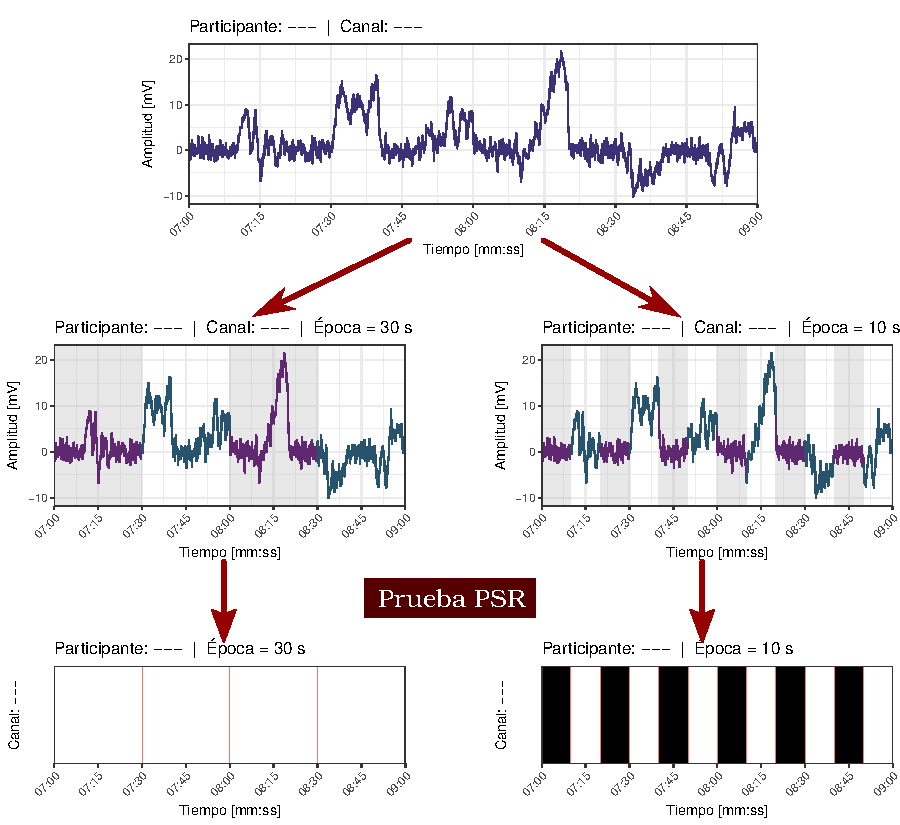
\includegraphics[width=\linewidth]{./img_diagramas/epocas_diferentes_v3.pdf}
\caption{Efecto del tamaño de ventana sobre la clasificación de estacionariedad.}
\label{epocas_diferentes}
\end{figure}

En otro ámbito, se replicó la metodología usada por McEwen \cite{McEwen75} para contrastar la afirmación de que las series de tiempo \textit{suficiente cortas} son estacionarias. 
%
Este procedimiento consistió en repetir la clasificación de épocas variando el tamaño de ventana; los tamaños de ventana se tomaron de la forma $30 \times 2^{n}$ segundos, para comparar con el tamaño de época recomendado por la AASM.

%%%%%%%%%%%%%%%%%%%%%%%%%%%%%%%%%%%%%%%%%%%%%%%%%%%%%%%%%%%%%%%%%%%%%%%%%%%%%%%%%%%%%%%%%%%%%%%%%%%
%%%%%%%%%%%%%%%%%%%%%%%%%%%%%%%%%%%%%%%%%%%%%%%%%%%%%%%%%%%%%%%%%%%%%%%%%%%%%%%%%%%%%%%%%%%%%%%%%%%
%%%%%%%%%%%%%%%%%%%%%%%%%%%%%%%%%%%%%%%%%%%%%%%%%%%%%%%%%%%%%%%%%%%%%%%%%%%%%%%%%%%%%%%%%%%%%%%%%%%
%%%%%%%%%%%%%%%%%%%%%%%%%%%%%%%%%%%%%%%%%%%%%%%%%%%%%%%%%%%%%%%%%%%%%%%%%%%%%%%%%%%%%%%%%%%%%%%%%%%